%% PNAStwoS.tex
%% Sample file to use for PNAS articles prepared in LaTeX
%% For two column PNAS articles
%% Version1: Apr 15, 2008
%% Version2: Oct 04, 2013

%% BASIC CLASS FILE
\documentclass{pnastwo}

%% ADDITIONAL OPTIONAL STYLE FILES Font specification

%\usepackage{pnastwoF}

\bibliographystyle{pnas2009}


%% OPTIONAL MACRO DEFINITIONS
%\def\s{\sigma}
%%%%%%%%%%%%
%% For PNAS Only:
%\url{www.pnas.org/cgi/doi/10.1073/pnas.0709640104}
%\copyrightyear{2008}
%\issuedate{Issue Date}
%\volume{Volume}
%\issuenumber{Issue Number}
%\setcounter{page}{2687} %Set page number here if desired
%%%%%%%%%%%%

\begin{document}

\title{Agreement on Characters and Characterization within Fandom Communities}

\author{Yizhi Jing\affil{1}{Indiana University Bloomington},
}

\contributor{2015Fall I590 Final Paper}

\maketitle

\begin{article}
\begin{abstract}
{This work studied the development of agreement on characterization of fictional characters within fandom communities, through analysis of transformative works that they produce. Based on data of a major fandom community that developed within the past a few years,  text analysis show that while writings about a character remain similar, changes of agreement in successive time periods may be observed. Meanwhile,  abstraction to the sentiment categories level indicates that although considerable divergence remains between authors, the agreement level tend to increase over time. Analysis with tags that summarize work contents suggest that while the time distribution of most frequent tags correlates mainly with the amount of works, tags that are favored most by community members have peaks in certain time periods that does not correspond to the overall distribution. Although higher popularity of tags does not necessarily lead to increased usage, this may imply the existence of diffusion processes within the community. }
\end{abstract}

\keywords{text analysis | sentiment analysis | cultural groups | information theory}

As one of the many types of dynamics in online communities, consensus of opinion captures multiple kinds of interaction, and exhibits different forms. In some communities, formal mechanisms for resolving discrepancies are provided: for example, Wikipedia keeps discussion pages for every entry, where editors attempt to reach agreement on how the entry should be written or modified. In such cases, it is easier to study the mechanism by collecting and analyzing empirical data systematically\cite{Kriplean:2007:CCC:1316624.1316648}. However, in many other situations, this process takes place in more subtle ways, and are more difficult to trace. 

In this work, I focus on a specific kind of online communities - fandoms. Fandom communities, by convention, are a group of people that identify, connect and interact with each other based on a similar interest, such as a movie, a book or a band\cite{wiki:fandom}. While many of the major events, such as comic-cons, happen offline, a large portion of fandom activities now takes place online.

Transformative works, or in a more common term, fan works, are one typical kind of production from fandom communities\cite{wiki:transf_work}. These are creative works made by fans based on one or more original works, and are often centered around certain characters or story lines. For example, a fiction written by a contemporary fan about Sherlock Holmes in his retirement is considered a fan fiction in the Sherlock Holmes fandom. By this nature, these works reflect the understanding of the authors about the characters and story, which differs from person to person and changes over time.

I base my work on the assumption that analysis of transformative works may reveal the development of consensus of opinion on characterization between fans. In particular, this development may be related to the typical life stages of a fandom, such as its origin, growth, decline and death. Intuitively, we may find two ways to describe this process that are both reasonable: it is possible that when the fandom grows and matures, common knowledge emerges between its members, and a higher level of agreement may be reached. However, it is also possible that as the size of the fandom increases, or because of other external events, more diversity will be introduced. It is this work's objective to formalize and verify these assumptions.

The data for this analysis comes from the online transformative work archive site Archive of Our Own (AO3)\footnote{\href{http://archiveofourown.org/}}. This site allows free host for works that users upload, and categorizes them based on fandoms. It also utilizes a metadata system to store these works' information, allowing for many filtering and classifying operations. Established in 2010, it has become one of the most popular transformative work archives.

As a starting point, the project is limited to only 1 fandom: \textit{Sherlock(TV) }, the BBC TV series starring Benedict Cumberbatch and Martin Freeman. It is chosen as the case for study because of two reasons: first, it is among the fandoms with largest amounts of data, covering $~3\%$ of all works on the site with 77, 510 works. Secondly, AO3 opened on January 1st 2010, while the first episode of \textit{Sherlock} was broadcasted  on July 2010\cite{wiki:sherlock}, which implies that the archive was able to record the life stages of the fandom since its origin.



\section{Method}
The data collected from the website includes 75,694 transformative works from the fandom described above, with publish dates ranging from July 2010 to November 2015. Count of words in this dataset is 405,230,386. 
Besides the work texts, the metadata collected includes 20 fields that can be roughly divided into two categories. One is tags generated by the author, which describes the work's content; the other is tags that are automatically generated, and describes the works' other information, as well as the readers' feedback. Table 1 gives the names of these fields. The time distribution of works published is shown in Figure  1\ref{time_work}, along with major events in the fandom, such as the broadcasting of a new season of the series. 

\begin{figure}
\centerline{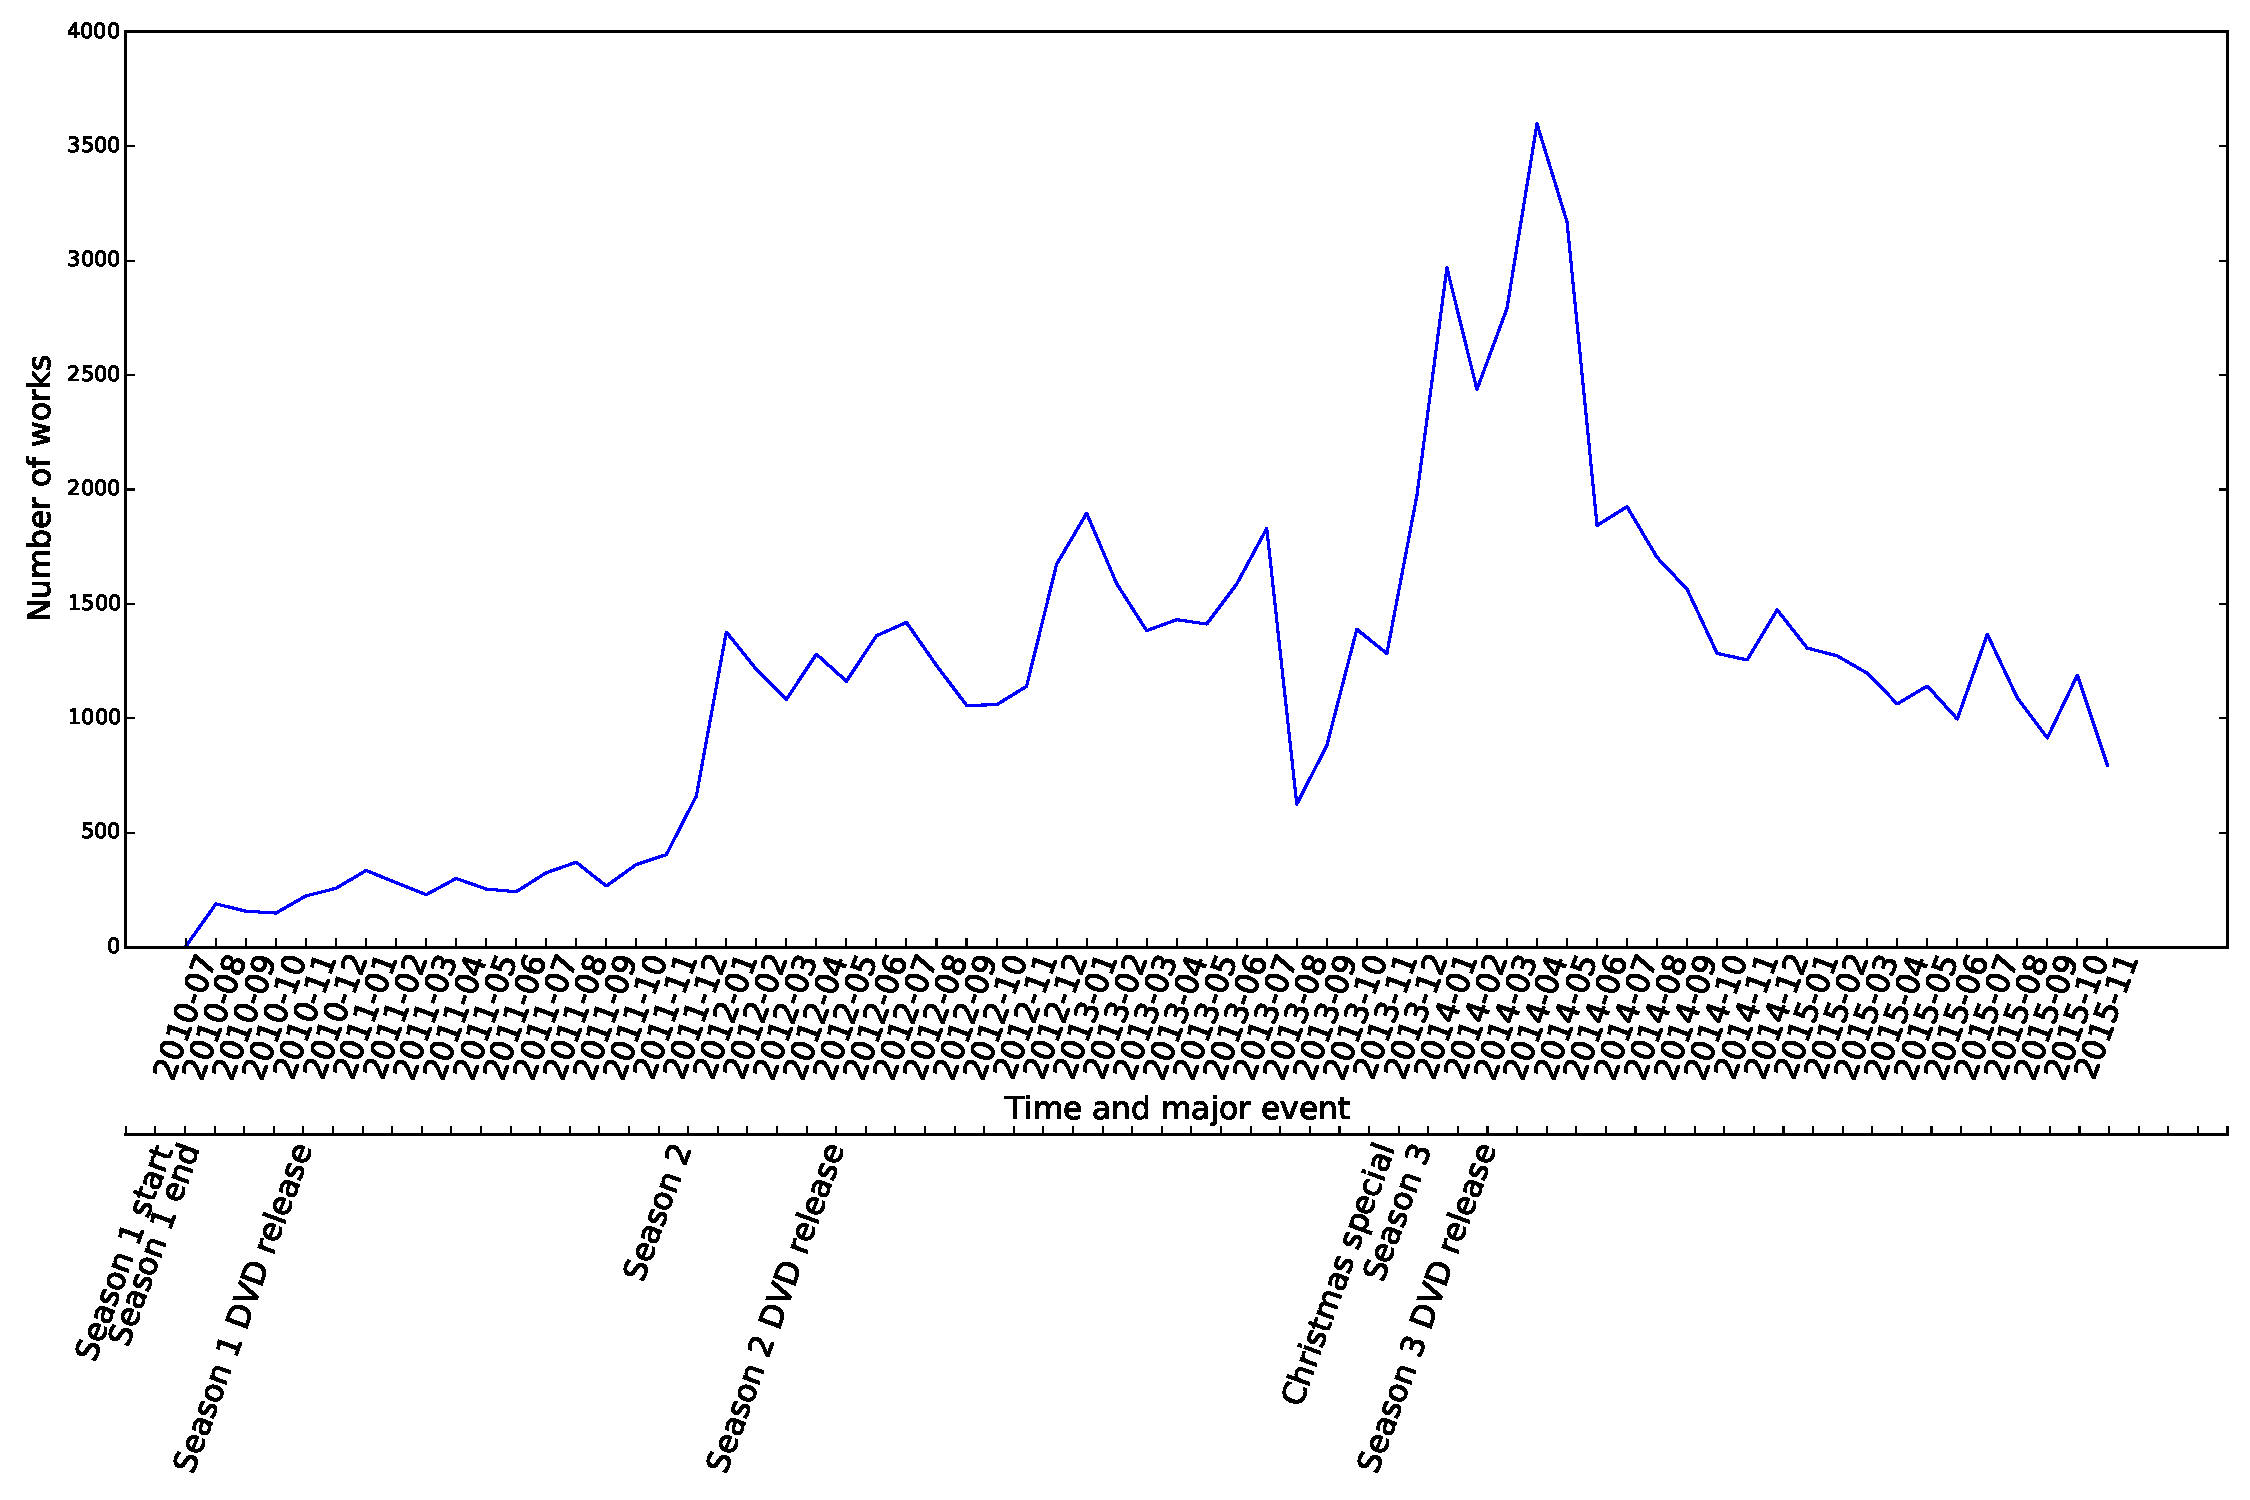
\includegraphics[width=.5\textwidth]{time_work.pdf}}
\caption{Time distribution of works published.}\label{time_work}
\end{figure}

The original plan includes extracting parts of the work texts that provides more information on characterization. There have been works that approach this objective, which mostly come from researchers in computational linguistics, narratology and morphology \cite{finlayson2012learning} \cite{noah2013learning}\cite{elsner2012character}\cite{chambers2009unsupervised}. However, it seems that current state-of-arts models are yet to provide simple and robust methods, and it may be risky to base further analysis on these results if complicated methods are introduced. Therefore, I chose to apply simpler methods, which focus on achieve a higher level of abstraction of the works and characters.

I first applied the word2vec algorithm to extract words that are most closely related to a given character. Introduced by Mikolov et al., this model has gained a lot of popularity in the past a few years\cite{mikolov2013efficient}. It trains a neural network with the given corpus, and is able to capture the words' context by creating a vector representation for each word. As a result, it is able to identify words that occur with similar patterns.

The works from the dataset are first grouped by their publish time (year/month), constructing subsets that correspond to slices of the time range, which includes 65 months. The average count of words per slice is therefore around 6 million, which may be a bit small for training a word2vec model. However, examination of the results suggest that it is able to capture similarities in a reasonable way. I then search for words that are mostly related to a given character (such as "Sherlock" or "Moriaty", and record the top 20 words for each subset. 

These word sets are then used to construct a document-word matrix, in which each  document consists of the top words from a subset of texts. To compare the change of similarity between works of different time periods, I chose to use the mutual information between two documents. Calculated as following, 

\begin{equation}
MI(X;Y) = \sum_{y\in Y}\sum_{x\in X} p(x, y) log(\frac{p(x,y)}{p(x)p(y)})
\end{equation}

This metric captures, in a sense, to what degree we can use one document to predict information about the other. 

Another possible approach to extract information from the texts to a more abstract level is through sentiment analysis. For this I applied the lexicon-based approach, which gives each word in the lexicon a score that describes its positiveness or negativeness. The lexicon used is from Mitchell et al's work that analyses Twitter's 
sentiment\cite{10.1371/journal.pone.0026752}, containing 10,000 commonly used words rated by Amazon Mechanical Turks. 

I then calculate the works' average sentiment scores by taking average over the words in the text that can be found in the lexicon, and categorize them into 3 categories (positive, negative and neutral). Following a similar approach in Elsner's work\cite{elsner2012character}, only sentences in which only a given character appears are considered.  For each time period, I record the number of works in the subset that are labeled as positive, negative and neutral, respectively. To estimate the agreement between authors, I calculate the Fleiss' kappa of these time periods\cite{wiki:fleisskappa} . Calculation for this metric is as following:

\begin{equation}
\kappa = \frac{\bar{P} - \bar{P}_e}{1-\bar{P}_e}
\end{equation}

Where $1-\bar{P}_e$ describes the degree of agreement that can be achieved above chance, and $\bar{P} - \bar{P}_e$ is the degree of agreement that is actually achieved above chance. In the calculation, each author is considered as a rater, and the kappa value captures the degree of agreement on the categories that their works fall into. 

Besides analysis on the text level, another approach is to work with the works' tags, which are found in the "Additional Tags" field of the metadata. These are created by the authors, and describes certain settings, memes and plots in a given work. In a sense, they are like tropes that captures specific narrative elements in the works. It seems possible that the popularity of a tag can be an indicator of how much community members are acceptive of it, and therefore, members' agreement on this particular element. The popular tags are identified in two ways: one is simply the frequency of its occurrence, and the second is to evaluate each tag by the kudos (likes) that works with this tag received on average, calculated as following:

\begin{equation}
p = \frac{\sum{K}}{n}
\end{equation}

Where $\sum{K}$ is the total number of kudos that works with this tag received, and n is the number of works with this tag. This data is found in the "Kudos" field of the metadata. In this case, tags are filtered by occurrence with a threshold of 100, as a way to reduce bias towards rare tags in works with extremely high Kudos. Some tags that may contain inappropriate contents are also filtered. 


\section{Results}
\subsection{Mutual Information} Figure 2 \ref{mi_pearson} shows the mutual information between every two successive months of words related to John Watson. The mutual information is adjusted against chance. Pearson correlation between each pair of word distributions are also plotted for comparison. It can be seen that while these two metrics correlates fairly well with each other (with correlation score of 0.92),  some difference in  patterns can also be observed.

To better understand the pattern of mutual information changes, I also calculate the mutual information between time periods with longer step lengths. The steps are defined as months, so that 2-step mutual information means the mutual information between this month and two months later, etc. Figure 3\ref{multi_mi} shows the 1-4 steps mutual information changes. It can be observed that the 2-step and 3-step comparisons are able to reveal a more clear pattern, showing a gradual increase and then fluctuating decrease. This may also suggest that a slightly longer time period, like 2-3 months, is a better unit to evaluate changes in the fandom community. 


\begin{figure}
\centerline{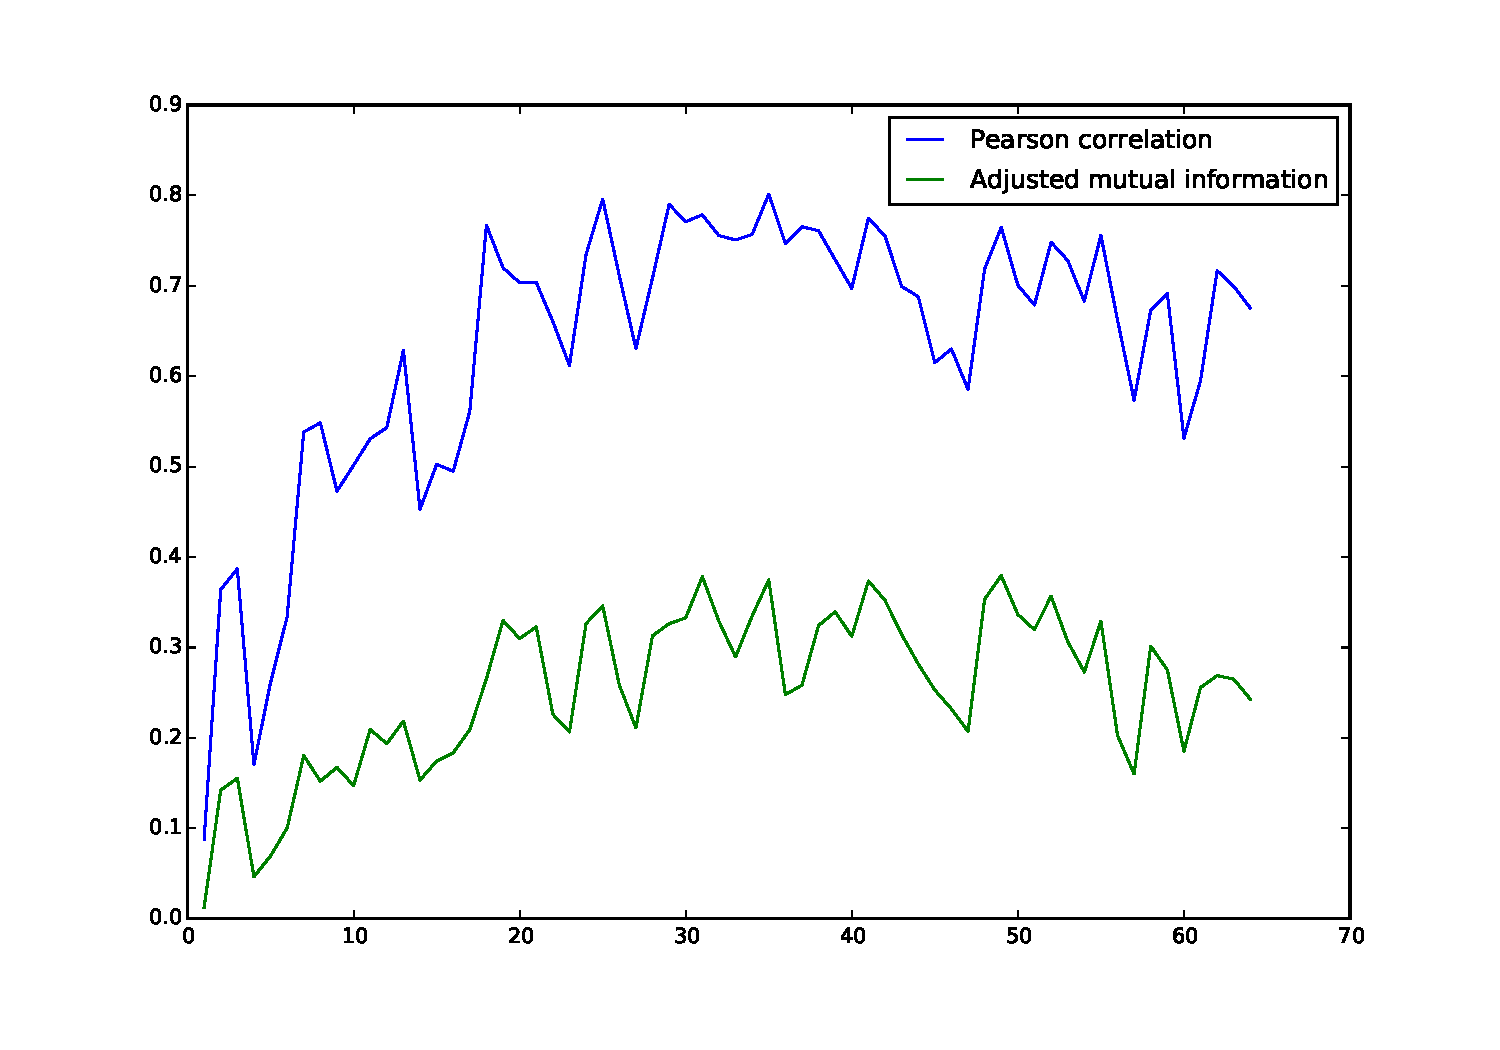
\includegraphics[width=.4\textwidth]{mi_pearson_watson.pdf}}
\caption{Adjusted mutual information and Pesrson correlation between word sets mostly related to John Watson during the time range.}\label{mi_pearson}
\end{figure}

\begin{figure}
\centerline{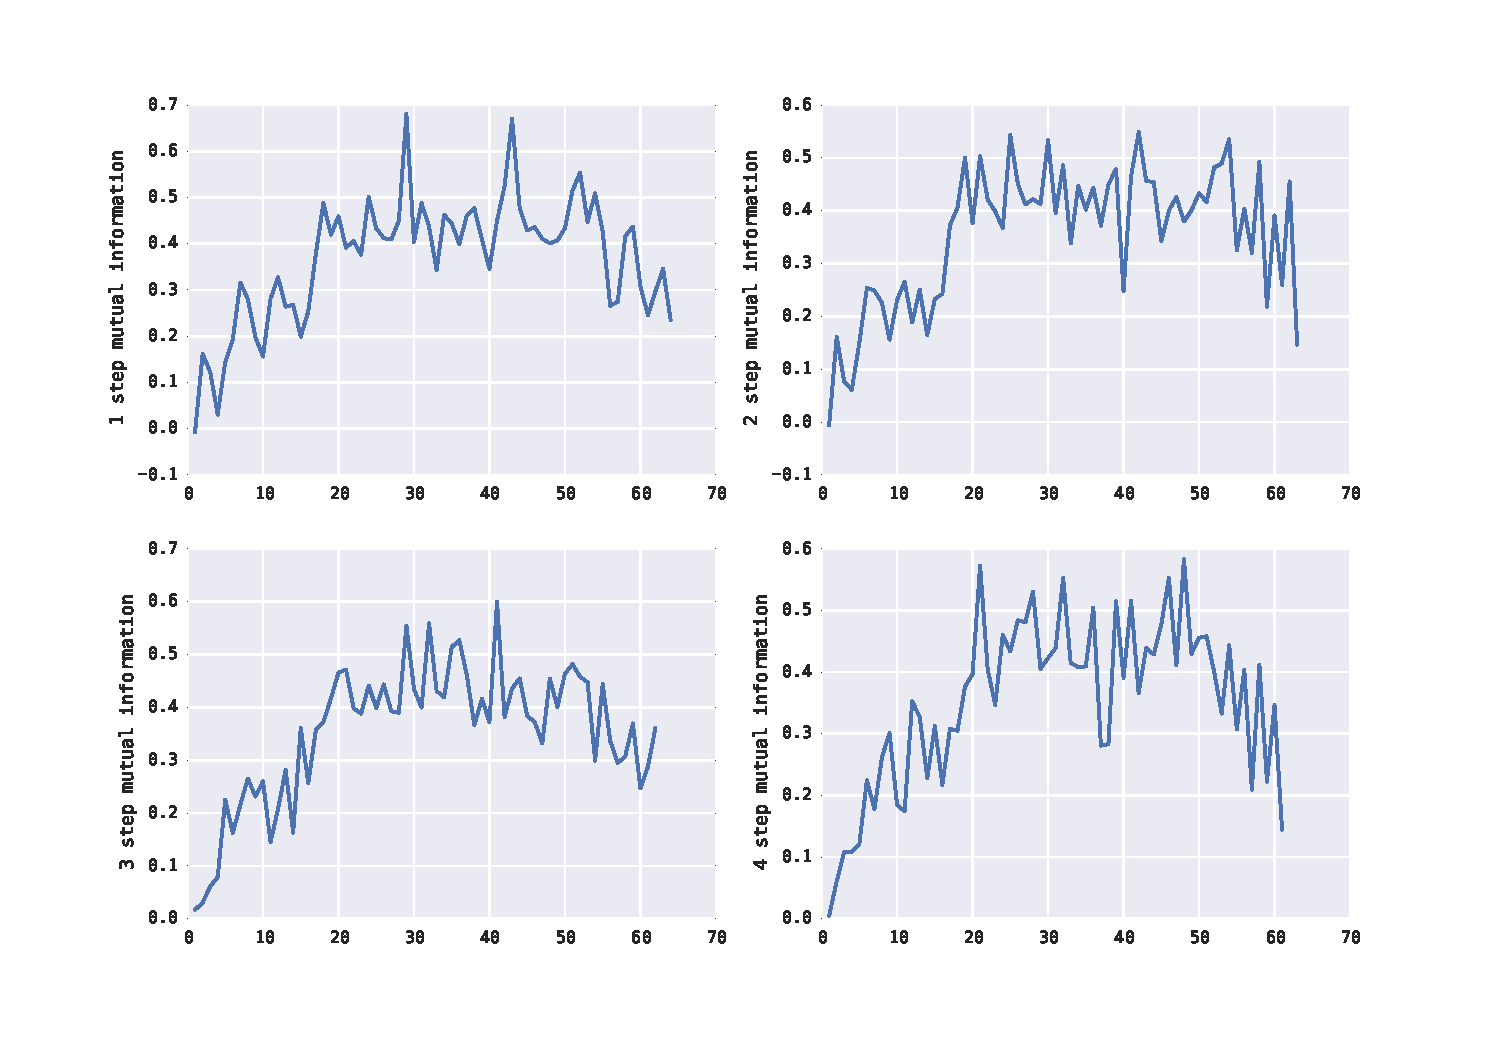
\includegraphics[width=.5\textwidth]{muti_step_mi_john.pdf}}
\caption{Adjusted mutual information between word sets mostly related to John Watson during the time range, with time step ranging from 1 to 4 months.}\label{multi_mi} 
\end{figure}


\subsection{Sentiment Analysis} The change of Fleiss' kappa between sentiment categorizations during the time range is shown in Figure 4 \ref{fleiss}, which focus on writings concerning Sherlock Holmes. It can be found that after the early period, agreement level quicily increased and stabilized at a certain level, but decreased slightly at the latest period.

Since the categories are subjectively divided, I also included a more fine-grained division of 10 categories, based on the sentiment score range of [1,10]. The difference in kappa values is minor, suggesting that the result is robust against different category divisions. However, it should also be noted that the agreement score remained slightly negative, which implies little agreement according to the conventional interpretation of this metric \cite{wiki:fleisskappa}. 


\begin{figure}
\centerline{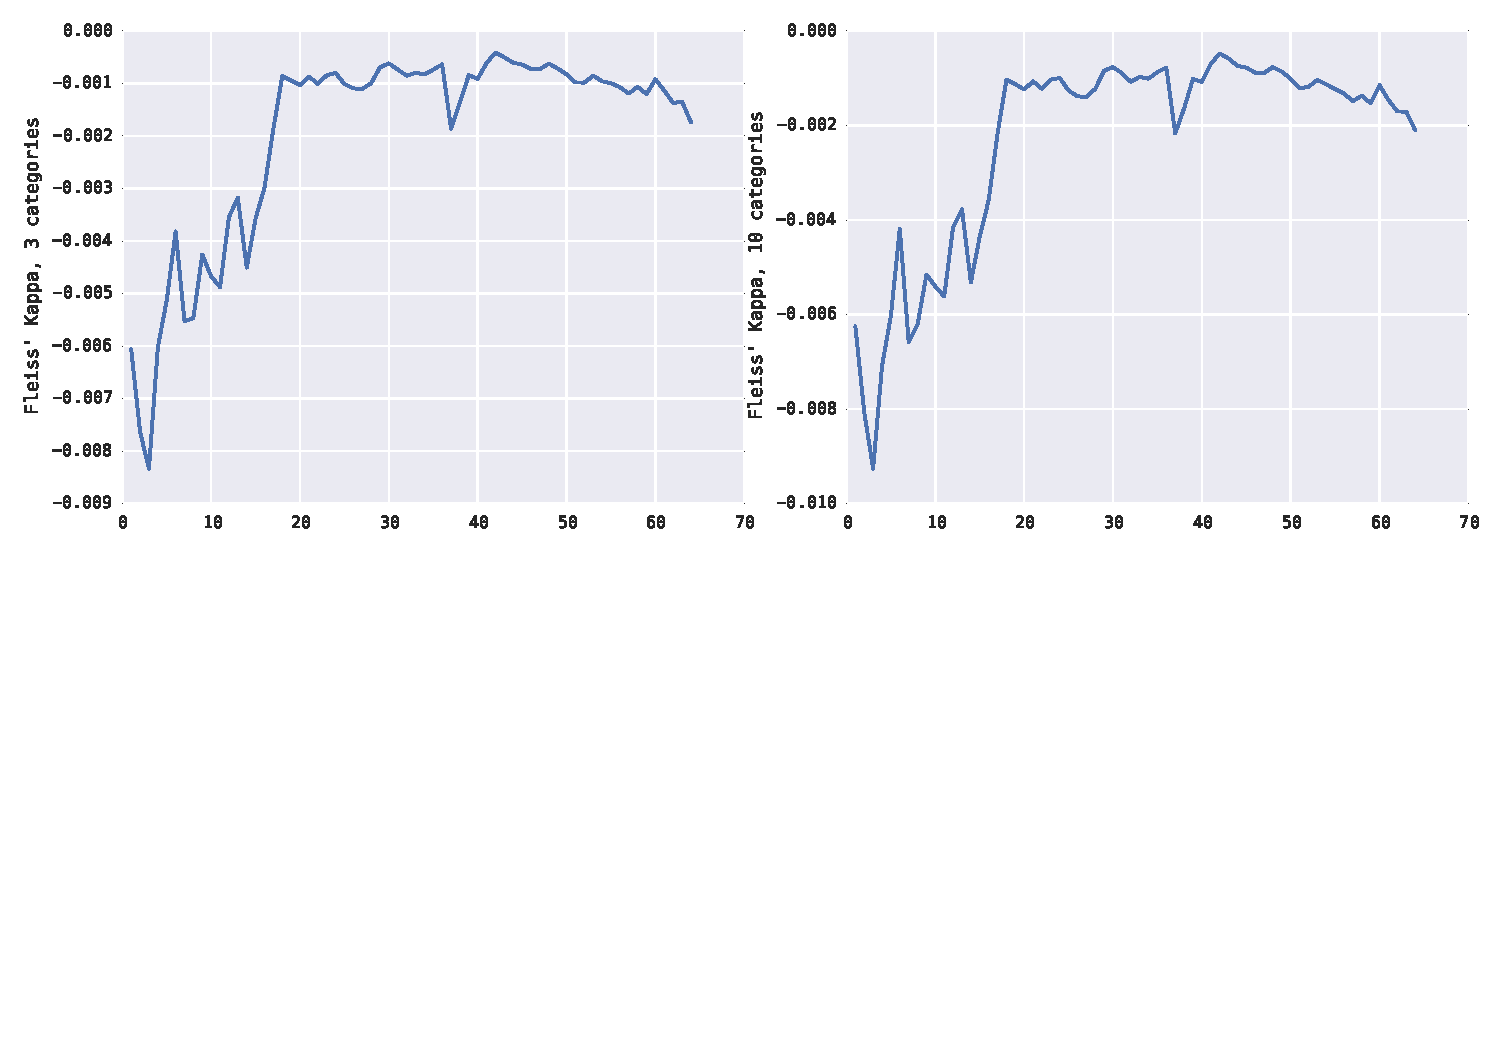
\includegraphics[width=.5\textwidth]{fleiss_kappa_3_10_categories.pdf}}
\caption{Fleisss' Kappa of sentiment categories of writings about Sherlock Holmes during the time range..}\label{fleiss}
\end{figure}


\subsection{Tag Analysis} Figure 5, 6 and 7\ref{freq_tag_wtotal} show the time distribution of the most popular tags, as identified by the method described above.  Figure 5 \ref{freq_tag} shows the top words with highest frequency. It can be immediately noticed that these tags' distributions respond directly to the total count of works, which is plotted in Figure 6\ref{freq_tag_wtotal} for comparison.

However, if we look at the tags that received most Kudos instead, as shown in Figure 7, the scenario becomes different. The distribution of most of these tags shows clear peaks that are centered around certain time periods, and occurrence decrease significantly after those periods. 

By looking more closely at these tags, we can notice that the tags with top frequency are mostly concerned with the overall genres of the works (such as ''angst' or 'humor'). Tags with most kudos, however, are concerned with specific tropes or story elements. As a result, the latter type captures the elements that gains most popularity during a certain time period. However, this popularity does not necessarily lead to a long-term increase of frequency of these tags.   

\begin{figure}
\centerline{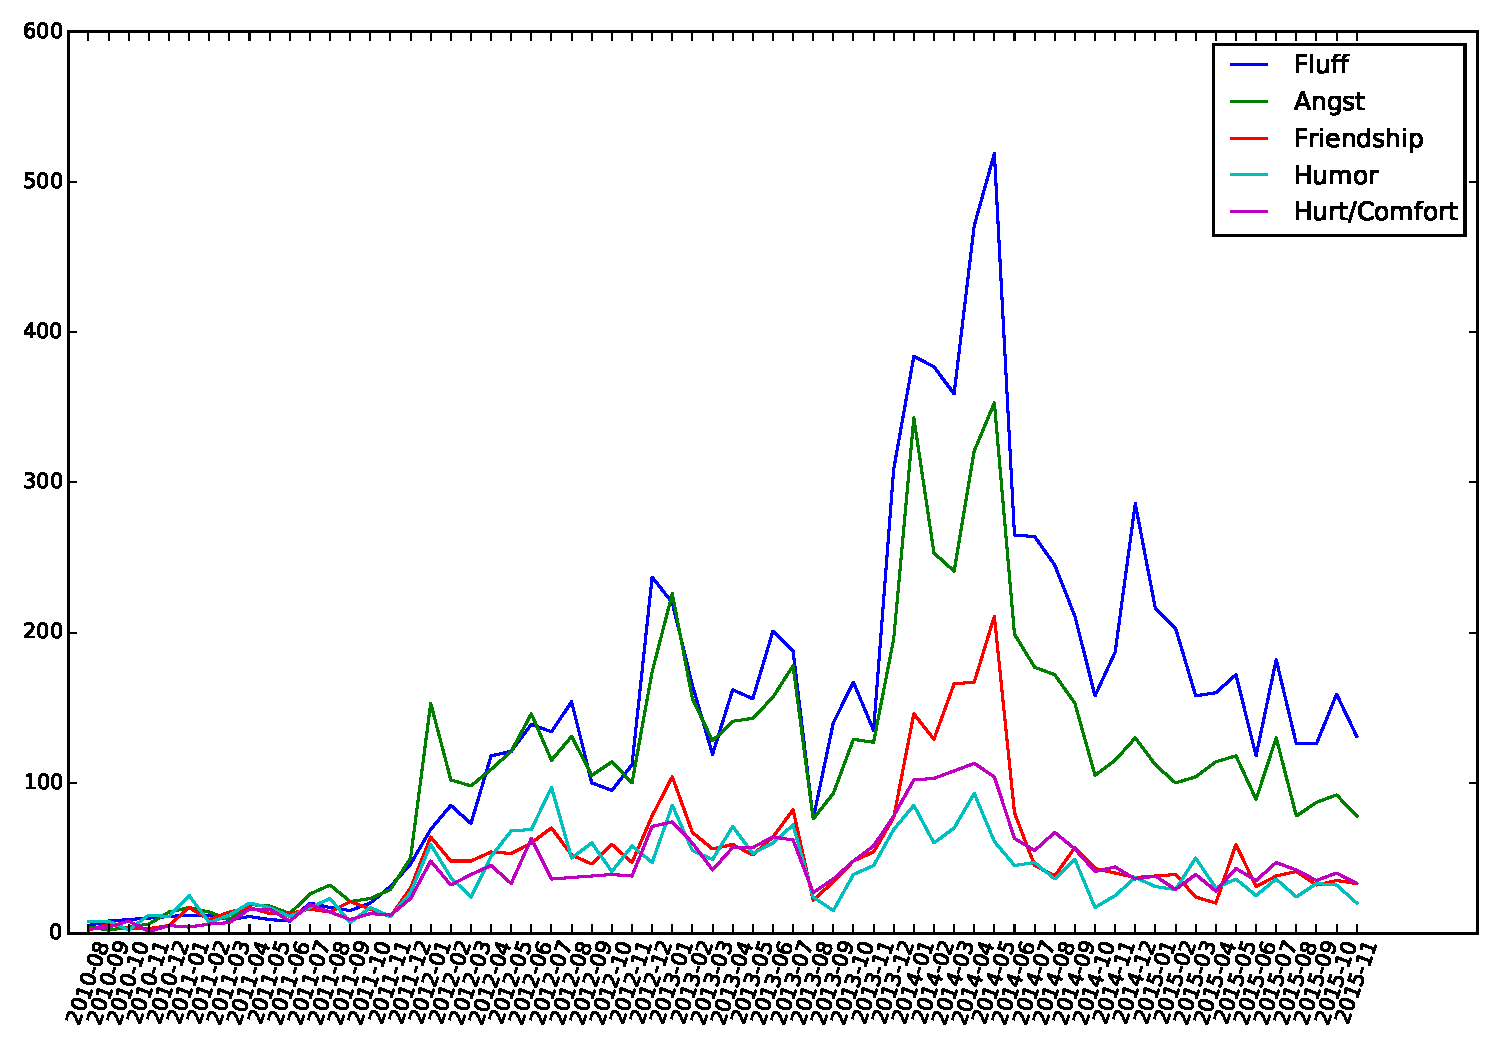
\includegraphics[width=.4\textwidth]{top_frequency_tag_time.pdf}}
\caption{Time distribution of top 5 tags according to total frequency of appearance.}\label{freq_tag}
\end{figure}

\begin{figure}
\centerline{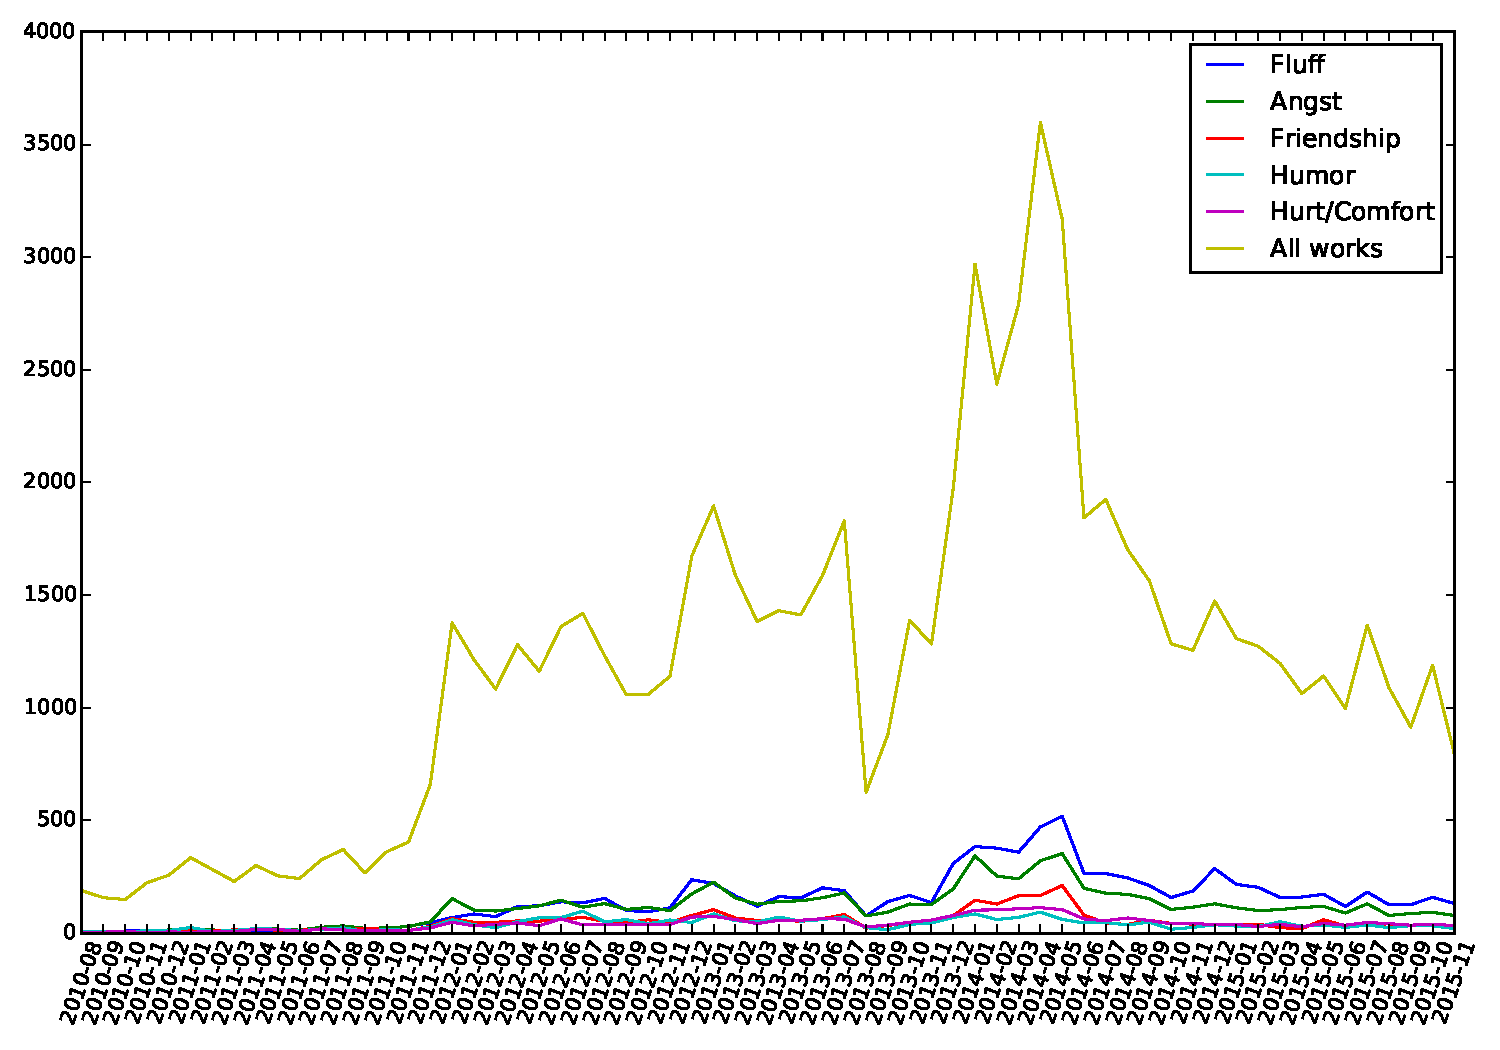
\includegraphics[width=.4\textwidth]{top_frequency_tag_time_w_total.pdf}}
\caption{Time distribution of top 5 tags identified by total frequency of appearance, with the total number of works.}\label{freq_tag_wtotal}
\end{figure}

\begin{figure}
\centerline{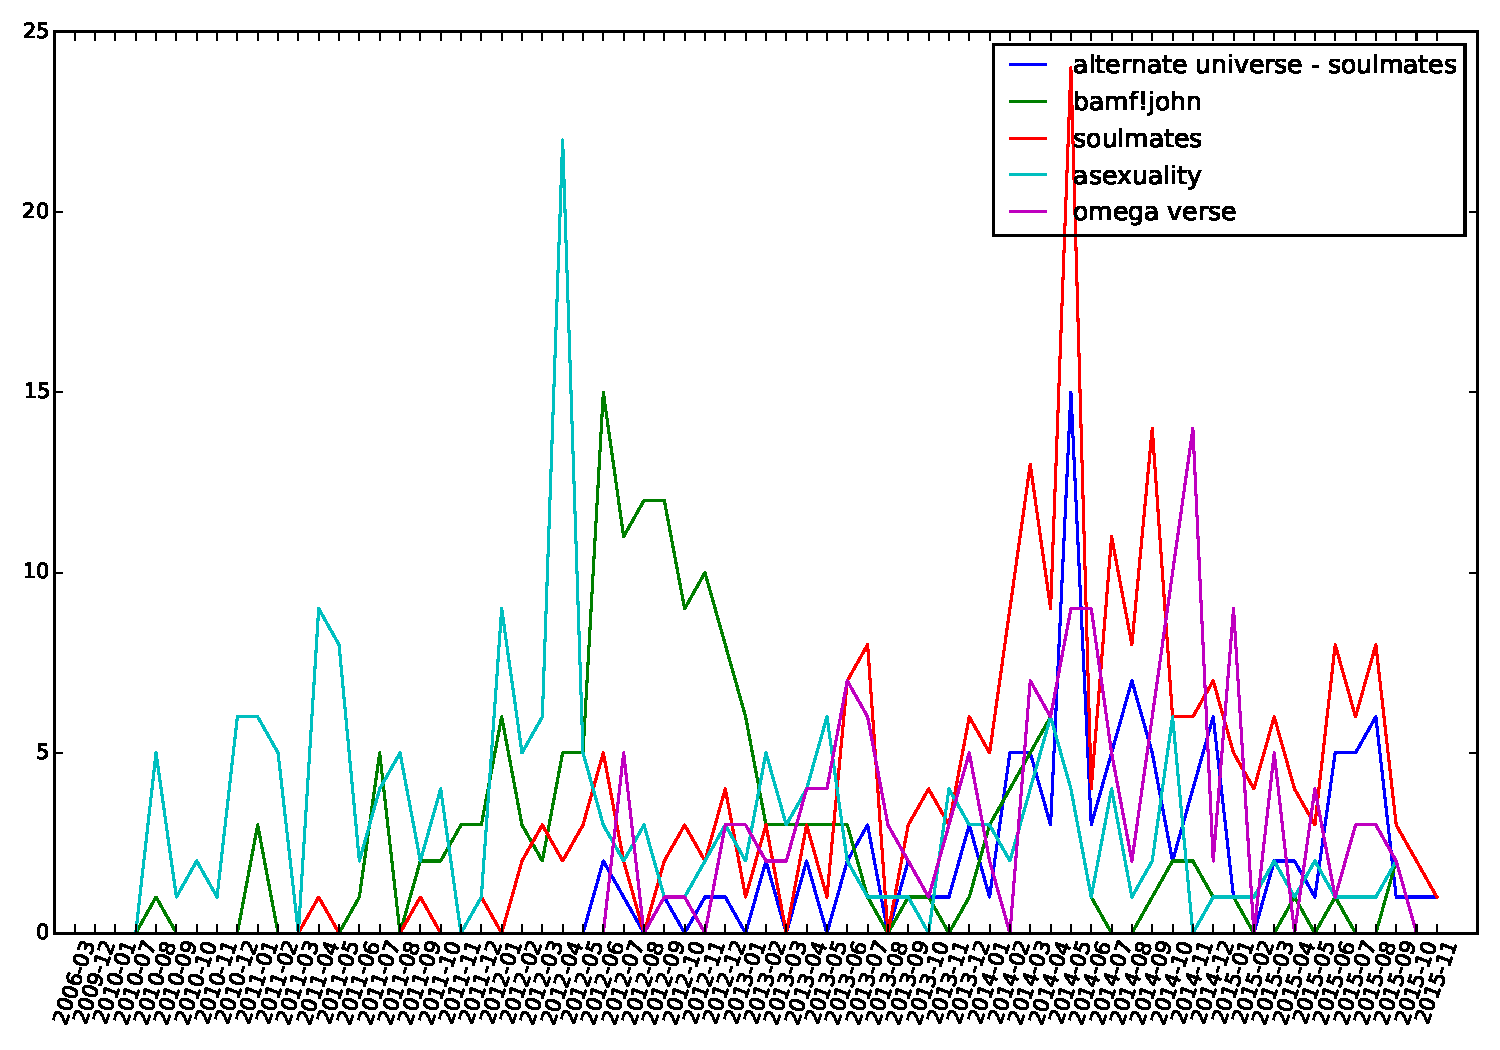
\includegraphics[width=.4\textwidth]{top_popularity_tag_time.pdf}}
\caption{Time distribution of top 5 tags identified by highest average Kudos.}\label{popular_tag}
\end{figure}

\section{Discussion and Conclusion}
The analysis presented above suggests that this dataset has been able to cover the major life stages of the fandom, including origin, growth, peak and decline, based the amount of transformative works produced. In this case, transformative works began to appear only a few days after the original work was first aired, and the amount of works continued to grow in the next three years, with peaks occuring every time a new season was broadcasted or DVDs were released. After the highest peak in early 2014, the amount of works began to drop significantly. (It is likely that we will observe a revival when the 4th season is aired in 2016, but this falls outside the concern of this work). 

It seems possible that the agreement on characterization is, in some ways, related to the development of the fandom. For example, from Figure 3 \ref{multi_mi} and Figure 4\ref{fleiss}, we are able to observe a significant change the origin and the mature period, in which the agreement level on top words related to characters and on sentiment categories  increased and stablized at a higher level. At the decline period, a slight decrease in both metrics can also be observed. 

This may imply that instead of a simple linear increase or decrease, the agreement on characterization is involved in a coevolution with the life stages of the fandom community. The level of agreement increases as the fandom grows and matures; and when the fandom starts to decline, noise and discrepancy once again rise, causing the level of agreement to drop as well. 

However, this observation also has a possible interpretation that the degree of agreement is simply related to the amount of works published, and this calls for the need to further investigate into the metrics applied to evaluate agreement. It is likely that this work will benefit from creating a baseline or ground truth collection for evaluation of the models. Besides, it is possible that the models can be improved by implementing methods that involve less curation, for if significant relations exist, they can probably be revealed by less complicated methods.

There are also a few topics that I would like to include in this work in the future. The most important part will be to extend the analysis to multiple fandoms, to see if similar patterns can be observed. It would also be interesting to take into account the number of authors, instead of the number of works, in each time period. With the tag analysis part, it is possible to introduce network analysis methods by constructing the co-occurrence network of tags, with which we can, for example, identify major clusters and important story elements.
 
\end{article}

\bibliography{I590_final_paper_yizhi_jing}

\begin{table}
\centering
\caption{Fields of AO3 work metadata}
\begin{tabular*}{\hsize}{@{\extracolsep{\fill}}lcr}
Metadata type&Fields\cr
\hline
Author generated&author, title, summary, fandom, \cr
 &characters, relationship, category, rating, \cr
 &additional tags, archive warnings, notes\cr
 \hline
System generated&publish date, complete date, chapter count,\cr
 & word count, bookmarks count, chapters count,\cr
  & hits, kudos, language, comment counts \cr
\hline
\end{tabular*}
\end{table}


\end{document}


